\section{Izmantotā darba platforma un rīki} \label{sec:devkit}
Par darbā izstrādāta mikrokontroliera kodola sintēzes platformu izmantots
\textbf{Actel Fusion Embedded Development Kit} uz kura izvietota
\textbf{Actel Fusion \texttt{M1AFS1500}} FPGA mikroshēma.

\begin{figure}[thb]
	\centering
	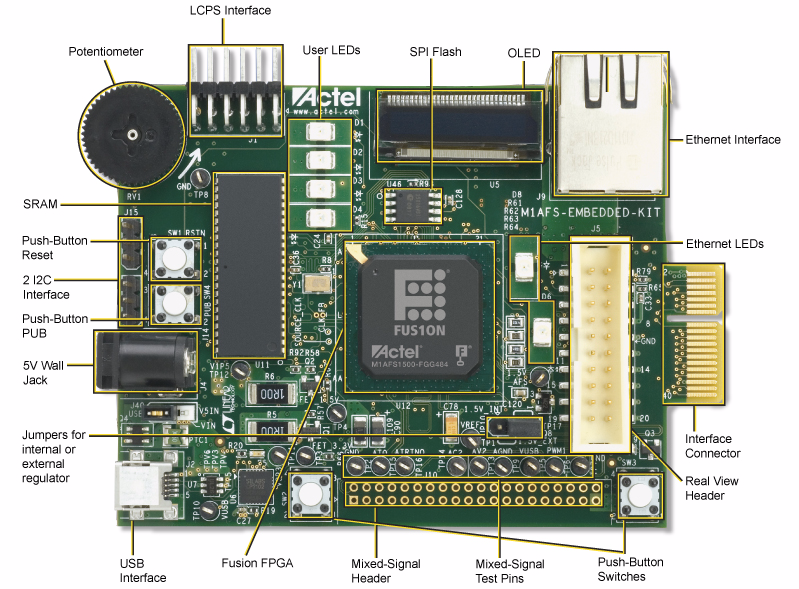
\includegraphics[width=0.8\textwidth]{devkit2}
	\caption[Actel Fusion Embedded Development Kit izstrādes platforma.]
			{Actel Fusion Embedded Development Kit izstrādes platforma \cite[7.~lpp.]{FusionGuide}.}
	\label{fig:devkit}
\end{figure}

Lai gan mikrokontroliera kodols ir izstrādāts platformas neatkarīgā VHDL,
parauga mikrokontroliera implementācija izmanto gan FPGA specifiskos
resursus, gan izstrādes platformas specifiskos resursus. Konkrēti, tika
izmantota uz izstrādes plates novietotā, 8 megabitu (512K mašīnvārdu)
ietilpības SPI \termEn{Flash} atmiņa \cite{FusionGuide}, kuras uzdevums ir uzglabāt 
pamatprogrammu (tās mašīnkodu).

Par darba vidi tika izmantota \textbf{Actel Libero IDE} programmpaka, kas
sevī iekļauj:
\begin{itemize}
	\item \textbf{Actel Libero} projekta pārvaldīšanai,
		kā arī HDL koda rediģēšanai un strukturālo komponenšu 
		grafisko shematiku zīmēšanai;
	\item \textbf{Mentor Graphics ModelSim} projekta darbības simulācijai
		un rezultātu (laika diagrammu) vizualizācijai;
	\item \textbf{Synopsis Synplify} projekta rezultāta sintēzei;
\end{itemize}

Papildus autors C un C++ valodā izstrādāja assembleri
 izstrādātā kodola instrukciju kopai mikrokontroliera mašīnkoda assemblēšanai.
